\chapter{리눅스 커널}
\section{리눅스 아키텍처}
\begin{itemize}
    \item \textbf{하드웨어 계층}\newline
        CPU와 메인 메모리, 디스크, NIC, I/O 디바이스 모두를 총칭한다.
    \item \textbf{커널 계층}\newline
        하드웨어 계층과 사용자 영역 계층의 사이에 위치한다.\newline
        이번 chapter에서 다루는 계층이다.
    \item \textbf{사용자 영역 계층}\newline
        shell 및 ps, ssh 같은 유틸리티, GUI를 비롯해 
        대부분의 앱이 실행되는 계층이다.
\end{itemize}

\begin{flushleft}
    다른 계층간 인터페이스는 리눅스 운영체제 패키지의 일부이다.
    그 중 커널과 사용자 영역 계층 인터페이스를 \textbf{시스템 콜}(system call)이라 부른다.
\end{flushleft}

\begin{flushleft}
    하드웨어와 커널 사이의 인터페이스는 시스템 콜과 달리 
    단일 인터페이스가 아니라 
    일반적으로 하드웨어별 그룹화된 개별 인터페이스 모음으로 구성된다.

    \begin{itemize}
        \item CPU 인터페이스
        \item main memory 인터페이스
        \item 네트워크 인터페이스와 드라이버
        \item 파일시스템과 블록 디바이스 드라이버 인터페이스
        \item 캐릭터 디바이스, 하드웨어 인터럽트, 
        키보드, 터미널, 기타 I/O 등의 입력 디바이스를 위한 디바이스 드라이버
    \end{itemize}
\end{flushleft}
\newpage

\begin{figure}
    \centering
    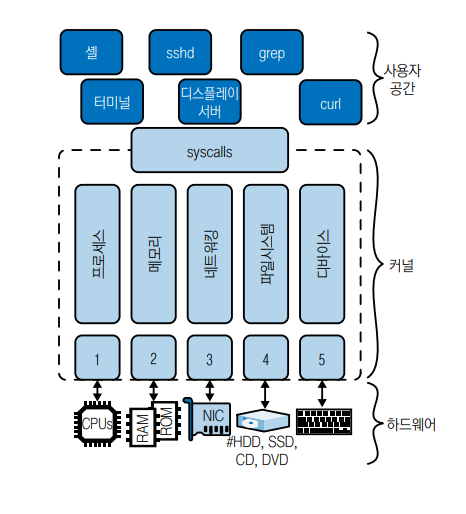
\includegraphics[width=10cm]{resource/2-1.png}
    \caption{리눅스 아키텍처 개요}
\end{figure}
\begin{flushleft}
    일반적으로 \textbf{커널 모드}는 추상화를 제한함으로써 빠르게 실행함을 의미하는 반면, 
    \textbf{사용자 모드}는 상대적으로 느리지만 더 안전하고 편리한 추상화를 의미한다.
    대부분의 경우 커널 모드를 신경쓰지 않아도 사용에 지장은 없지만, 
    커널과 상호 작용하는 방법(시스템 콜)을 아는 것은 중요하다.
\end{flushleft}


\section{CPU 아키텍처}
\subsection{x86-64 아키텍처}
\begin{flushleft}
    x86과 amd64를 합쳐서 x86-64라고 부른다. 
    x86은 인텔 32-bit ISA이며, amd64는 64-bit ISA이다.
    대부분의 경우 사용되는 CPU이며 오래전부터 사용되어왔고, 
    CISC(Complex Instruction Set Computer) 아키텍처 에너지 효율은 높지 않다.
\end{flushleft}

\subsection{ARM 아키텍처}
\begin{flushleft}
    RISC(Reduced Instruction Set Computer) 아키텍처이며 적은 명령어 집합을 사용한다.
    RISC는 CISC에 비해 전력 소모가 적다는 장점을 가지고 있으며, 
    저전력 환경(임베디드, 휴대용 디바이스)에서 널리 사용된다.
\end{flushleft}


\subsection{RISC-V 아키텍처}
\begin{flushleft}
    ARM과 달리 개방형 RISC 표준으로 아직 널리 사용되지는 않는다. 
    다만 ARM과 달리 라이센스 비용이 없어 주목받고 있다.
\end{flushleft}


\section{커널 구성요소}
커널 코드에서 제공하는 주요 기능은 다음과 같다.

\begin{itemize}
    \item \textbf{프로세스 관리}: 실행 파일을 기반으로 프로세스 시작
    \item \textbf{메모리 관리}: 프로세스에 메모리 할당 및 파일을 메모리에 매핑
    \item \textbf{네트워킹}: 네트워크 인터페이스 관리 및 네트워크 스택 제공
    \item \textbf{파일시스템}: 파일 관리를 제공하고, 파일 생성과 삭제 지원
    \item 케릭터 디바이스와 디바이스 드라이버 관리
\end{itemize}

\subsection{프로세스 관리}
\begin{itemize}
    \item \textbf{세션}\newline
        하나 이상의 프로세스 그룹을 포함하고 선택적으로 tty가 연결된 
        상위 수순의 사용자 대면 유닛.
        커널은 textbf{세션 ID}(SID)라는 번호를 통해 세션을 식별한다.
    \item \textbf{프로세스 그룹}\newline
        하나 이상의 프로세스가 포함되어 있으며, 
        한 세션에는 foreground 프로세스 그룹이 둘 이상일 수 없다.
        커널은 \textbf{프로세스 그룹 ID}(PGID)라는 숫자를 통해 프로세스 그룹을 식별한다.
    \item \textbf{프로세스}\newline
        여러 리소스(주소 공간, 하나 이상의 스레드, 소켓 등)를 그룹으로 추상화한 것이며, 
        커널은 /proc/self를 통해 현재 프로세스를 사용자에게 노출한다.
        커널은 \textbf{프로세스 ID}(PID)라는 숫자를 통해 프로세스를 식별한다.
    \item \textbf{스레드}\newline
        커널에 의해 프로세스로 구현된 유닛을 말한다.
        즉 스레드를 나타내는 전용 데이터 구조는 없다.
        오히려 스레드는 특정 리소스(ex - 메모리, signal handler)를 다른 프로세스와 공유하는 프로세스다.
        커널은 \textbf{스레드 ID}(TID)와 \textbf{스레드 그룹}(TGIO)를 통해 스레드를 식별하며, 
        공유된 TGID 값은 멀티스레드 프로세스를 의미한다.
    \item \textbf{태스크}\newline
        커널에는 sched.h에 정의된 \textbf{task\_struct}라는 데이터 구조가 있으며, 
        이는 프로세스와 스레드 구현의 기반을 형성한다.
        이 데이터 구조는 스케줄링 관련 정보, 식별자(ex - PID, TGID), signal handler, 
        성능이나 보안과 관련된 기타 정보를 수집한다.
        즉, 앞서 언급한 모든 유닛은 태스크에서 파생되거나 고정(anchor)된다. 
        하지만 캐스크는 커널 외부에 그대로 노출되는 일이 없다.
\end{itemize}

\begin{flushleft}
    실제로 그러한지 실습해보자.\newline
    아래는 ps -j로 확인할 수 있는 정보이다.
\end{flushleft}

\begin{figure}[h]
    \centering
    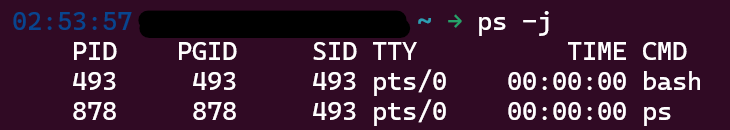
\includegraphics[width=10cm]{resource/ps-example.png}
    \caption{실습}
    \begin{enumerate}
        \item bash 셸 프로세스의 PID, PGID, SID는 모두 -이다.\newline
            ls -la /proc/493/task/493/로 태스트 수준의 정보를 수집할 수 있다.
        \item ps 프로세스의 PID/PGID는 878이고 SID는 셀과 동일하다.
    \end{enumerate}
\end{figure}

\begin{figure}
    \centering
    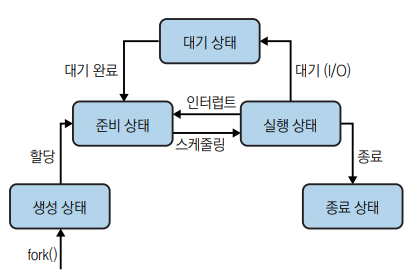
\includegraphics[width=10cm]{resource/2-2.png}
    \caption{리눅스 프로세스 상태}
\end{figure}


\subsection{메모리 관리}
작성예정

\subsection{네트워킹}
리눅스의 네트워크 스택은 계층화된 아키텍처를 따른다.

\begin{itemize}
    \item \textbf{소켓}\newline
        추상화 커뮤니케이션을 위해 필요
    \item \textbf{TCP(Transmission Control Protocol) 및 UDP(User Datagram Protocol)}\newline
        각각 연결형 통신과 비연결형 통신
    \item \textbf{인터넷 프로토콜}(IP)\newline
        기기의 주소 지정을 위해 필요
\end{itemize}

\begin{flushleft}
    이와 같은 세 가지 작업은 커널이 처리하는 모든 것이다.
    HTTP나 SSH 같은 애플리케이션 계층 프로토콜은 주로 사용자 영역에서 구현된다.
\end{flushleft}

\subsection{파일시스템}
\begin{flushleft}
    리눅스는 파일시스템을 사용해 HDD, SDD, 플래시 메모리 같은 
    저장 디바이스의 파일과 디렉터리를 구성한다. 
    ext4, btrfs, NTFS 같은 다양한 융형의 파일시스템이 있으며 
    동일한 파일 시스템의 인스턴스도 여러 개 사용할 수 있다.
\end{flushleft}
\begin{flushleft}
    가상 파일시스템(Virtual File System, VFS)은 원래 여러 파일시스템 유형과 인스턴스를 지원하기 위해 도입되었다.
    VFS의 최상위 계층은 열기, 닫기, 읽ㄱ, 쓰기 기능 등 공통 API 추상화를 제공하며, 
    VFS의 최하위 계층은 주어진 파일시스템에 대한 \textbf{플러그인}이라고 불리는 파일시스템 추상화다.
\end{flushleft}

\subsection{디바이스 드라이버}
작성 예정

\subsection{시스템 콜}
작성 예정

\section{커널 확장}
작성 예정

\subsection{모듈}
작성 예정

\subsection{커널을 확장하는 현대적인 방법: eBPF}
작성 예정